\documentclass[12pt]{article} 
%\geometry{verbose,letterpaper,tmargin=2.54cm,bmargin=2.54cm,lmargin=2.54cm,rmargin=2.54cm} 
\usepackage[backend=bibtex,style= ele,natbib=true]{biblatex}
\addbibresource{Stable_Isotopes_and_Fatty_acids.bib} 

\usepackage{graphicx}

\begin{document}


\title{Supporting Information S2: Maximizing resolution and computational efficiency - selecting fatty acids for analysis}
\maketitle

\section{Selecting fatty acids for diet analysis: an ordination approach}
Given the data transformations applied in our model, choosing a large
number of fatty acids (FAs) becomes computationally
prohibitive. Although model complexity scales with the number of FAs,
individual predators and prey species, transformation of FAs disproportionately affect computation time. It is thus inevitable to
choose an appropriate subset of FAs for diet analysis. When FA
profiles are obtained (typically from gas chromatography), the
practitioner faces the choice of which FAs out of the potentially
large number of measured FAs to retain for the analysis of diet
proportions. Typically, only few fatty acids will be informative about diets by separating sources in multivariate space. Adding FAs beyond these informative FAs does not improve estimates of diet proportions, but may instead increase colinearity among prey samples, adding more within-prey variance and thereby make discrimination more difficult.

While most studies quantify and list the most abundant FAs, these may
not be the most informative to discriminate among potential prey
species. Choosing FAs with experimentally validated conversion
coefficients is another important consideration. Eliminating FAs with
conversion coefficients that are unknown and suspected to be far from
1 is an important first step since their inclusion can introduce
significant uncertainty and error in point estimates. Once this
preliminary sorting is complete, we propose to select variables based
on their contribution to axes in a constrained ordination. We
specifically use Constrained Analysis of Principal Coordinates
\citep{anderson_canonical_2003} since it can deal with any distance
metric, and use compositional distance as a distance metric for
ordination \cite{aitchison_logratio_2000}. For each FA $f$, we sum over
the product of the FA contribution to the ordination axes and the
axes’ respective eigenvalues: $A_f = \sum_{a=1}^{n-1} \lambda_a
c_{f,a}$, where $a$ indexes individual ordination axes, and $c_{f,a}$ is the
contribution of FA p$f$ to axis $a$. Each $A_f$ then contributes a
proportion $p$ to $A=\sum_f A_f$, and we can sort $A_f$ and choose a
number of variables that contribute to a cumulative proportion $P$ of the
cumulative separation $A$.

To test this approach to selecting variables in a FAP, we simulated
75 separate datasets of three potential prey species (40 samples each) and six individual
predators, each with FAP of 20 individual FAs. Source separation was
randomly drawn, but with a large enough mean to assure that with the
full dataset estimation of diet proportions should be accurate. We ran the fatty acid 
mixing model for each simulation using reduced FA subsets that accounted for at least 75\%, 85\%
90\%, 95\%, 98\% and 99\% of the cumulative source
separation. Although we used
default priors for each analysis, which may lead to sub-optimally
parametrised models, we used relative errors within simulated datasets
as a measure of relative performance of FA subsets to avoid between
simulation comparisons that would be biased by this \emph{ad-hoc}
parametrization. Errors were calculated as compositional distance of
posterior means for estimated proportions from
the simulated composition \cite{aitchison_logratio_2000}, where again
only relative distances within a simulated data-set are
relevant.

\section{Selecting fatty acids for diet analysis: simulation results}

Our simulations confirm that selecting variables will impact
estimation accuracy by decreasing accuracy on average, for individual
simulated datasets the effect was difficult to predict. Prey
colinearity in FA space is likely to blame.

In practice, the amount of useful variation (between prey variance) discarded by variable selection will be a major determinant of how well the variable selection approach works. If prey items are difficult to discriminate even with a great number of FAs, then variable selection may discard useful information and estimation accuracy will decrease as a result. Grouping prey items into relevant groups (e.g., species into orders, or higher taxonomic groupings) is a popular approach that may eliminate such problems in many situations, allowing for meaningful variable selection to discriminate among remaining groups of prey.


\quad
\begin{figure}[!htbp]
  \begin{center}    
      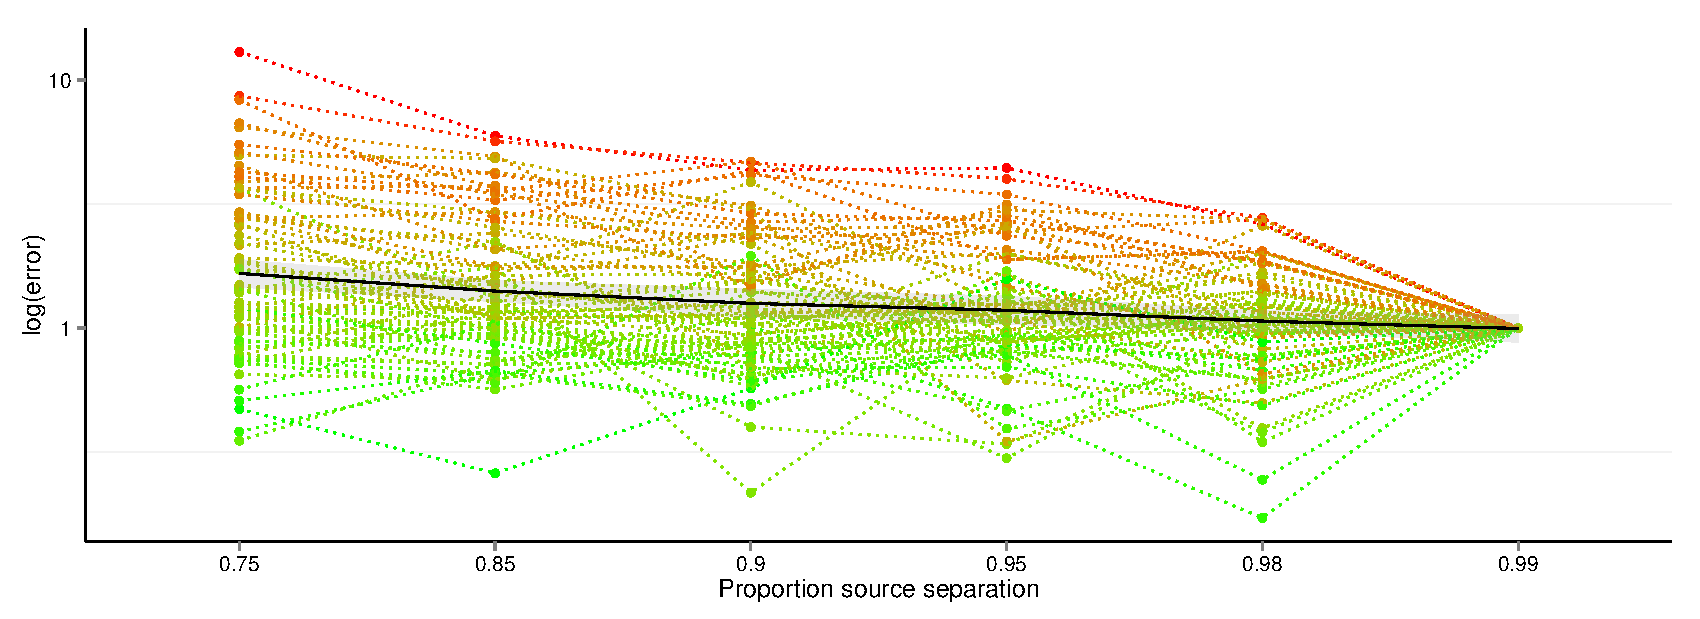
\includegraphics[width=0.75\textwidth]{Simulations/figures/test_var_select.pdf}  
       \caption{Relative errors in estimated posterior mean diet
         proportions, as a function of percent between source
         variation retained during variable selection. Errors are
         relative to estimated diet proportions with 99\% variance retained.}
\label{fig:test_var_select}
\end{center}
\end{figure}
\quad

\printbibliography

\end{document}